The Taylor shift by $a$ of a polynomial $P$ consists on evaluating the coefficients of $P(x+a)$. So, for a polynomial $P=\sum_{0\leq i \leq n} f_i\,x^i\, \in \, \mathbb{Z}[x]$ and $a\in\mathbb{Z}$, we want to compute the coefficients $g_0,\,\dots,\,g_n\,\in\,\mathbb{Z}$ of the Taylor expansion :

$$Q(x)=\sum_{0\leq k \leq n}g_k\, x^k=P(x+a)=\sum_{0\leq i \leq n}f_i\, (x+a)^i$$ 

There exists several classical polynomial arithmetic methods and also asymptotically fast methods described in \cite{Gerhard}. Among the three classical polynomial arithmetic methods explained in \cite{Gerhard}, all these methods amount to deal with the Horner's method to do a Taylor shift by 1. We have already explained in what consists this method in the part Horner's rule. I implement the Horner's method in C++ code, see appendix for this code.\\

Concerning the asymptotically fast methods, if we take a look at the different execution times, we remark that the divide and conquer (D \& C) method is the fastest one. This is the method we favour for parallel programming. I implement also a melt of the convolution method and the D \& C method in C++ code, just to have a preview of the result and compare it with the Horner's method and the D \& C method in parallel. I don't develop so much this method for the reason I had implement the Horner's method and it was sufficient to compare with the parallel method. In our work we mainly want to do a Taylor shift by $1$.

\subsection{Divide \& Conquer method (D \& C)}
This method consists to split a polynomial $P$ of degree $n=2^e-1$ (so this polynomial as $2^e$ coefficients) in other polynomials we split also. We will call \textit{size of a polynomial} the number of coefficients of this polynomial, so we consider here polynomials of size a power of $2$. We split the polynomial considered as the following (for a Taylor shift by 1) :\\

At the beginning, we split $P$ like this :

$$P(x) = P^{(0)}(x+1)+(x+1)^{\frac{n+1}{2}}\times P^{(1)}(x+1)$$

Then, we evaluate $P^{(0)}(x+1)$ and $P^{(1)}(x+1)$ recursively. So we have finally to consider 3 things, the computations of all the $(x+1)^{2^i}$ for $i\in \mbox{\textlbrackdbl} 0, e-1\mbox{\textrbrackdbl}$, a multiplication of one of these $(x+1)^{2^i}$ with the evaluation of a $P^{(j)}(x+1)$ and then an addition. One may notice that :\\
\begin{itemize}
\item[\textbullet] We just need all the taylor shift by 1 of the monomial $x^{2^i}$ for $i\in \mbox{\textlbrackdbl} 0, e-1\mbox{\textrbrackdbl}$, namely $(x+1)^{2^i}$.
\item[\textbullet] At each step, we split polynomials of size $2^d$ in two polynomials of size $2^{d-1}$, so at each step of the recursion, we approach a size which will be more and more easier to compute (and the size is always a power of 2).
\item[\textbullet] Contrary to the polynomial $P^{(j)}$ we consider, $(x+1)^{2^i}$ is not a power of $2$ (except for $i=0,1$). This will be a problem we will need to solve later, and we will see why and what's our strategy.
\item[\textbullet] At the next step of this recursion, we call the coefficients of $P(x)$.\\
\end{itemize}

We can represent how to do this recursion as the following tree. At the beginning we want to split the polynomial $P(x+1)$ not evaluated in two polynomials, which need to be splitted in turn, and so on. So the recursion begin at the top of this tree.

\begin{center}
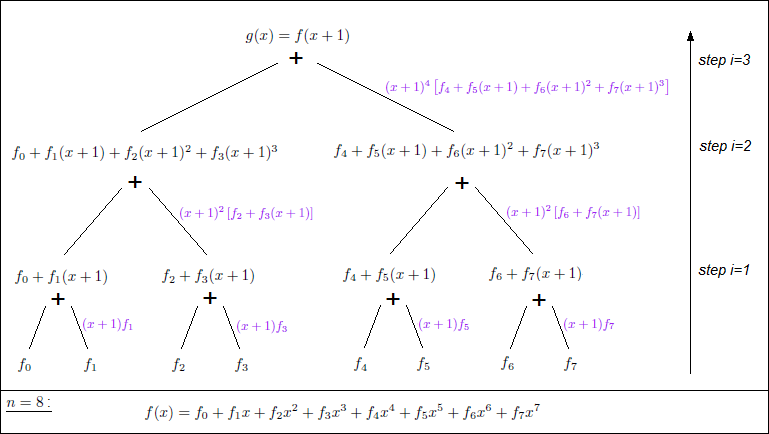
\includegraphics[scale=0.8]{ComputingTree.png}
\end{center}

The first problem we can encounter is the fact it is not simple to make a recursive algorithm in parallel. That's why finally we will consider the tree since its base, i.e. from the coefficients of the input polynomial coefficients. In the C++ code, I did the recursive method, and it was easier to write a method from the base in parallel. In each branch, we see if we need to multiplicate the polynomial evaluated at the base by a monomial shift or not. We see that for each step, the parallelism can be obtained easily. Now the difficulty is to work step by step, consider the good sizes of the arrays, the number of polynomials, the position of the coefficients we're modifying, how to do that the fastest possible.
